\documentclass[10pt]{article}

\def\Type{LessonCaelan}
\def\TypeNum{Lesson 22}
\def\TypeTitle{Expectation and Variance}
\def\Semester{Fall 2021} %Not Used 
\def\Course{MATH 1190 \& 1210}

\usepackage{preambleDJ}


%%%%%%%%%%%% BEGIN DOCUMENT %%%%%%%%%%%%%%%
%%%%%%%%%%%% BEGIN DOCUMENT %%%%%%%%%%%%%%%
%%%%%%%%%%%% BEGIN DOCUMENT %%%%%%%%%%%%%%%
%%%%%%%%%%%% BEGIN DOCUMENT %%%%%%%%%%%%%%%
%%%%%%%%%%%% BEGIN DOCUMENT %%%%%%%%%%%%%%%

%%%%%%%%%%%% BEGIN DOCUMENT %%%%%%%%%%%%%%%
%%%%%%%%%%%% BEGIN DOCUMENT %%%%%%%%%%%%%%%
%%%%%%%%%%%% BEGIN DOCUMENT %%%%%%%%%%%%%%%
%%%%%%%%%%%% BEGIN DOCUMENT %%%%%%%%%%%%%%%
%%%%%%%%%%%% BEGIN DOCUMENT %%%%%%%%%%%%%%%



\begin{document}

\thispagestyle{firstpage}
\pagestyle{otherpages}
\vs{0.4}

%\Heading{MATH 1190 \& 1210 Survey of Calculus I}{\begin{minipage}{0.25\textwidth}\begin{center} Lesson 20\\ Introduction to Probability \end{center}\end{minipage}}

\textbf{Intended Learning Outcomes}
After this lesson, you will be able to 

\begin{itemize}
    \item Define and explain the meaning of expectation and variance. (\target{P1, P2})
    \item Find the expectation and variance of a discrete random variable. (\target{P1})
    \item Find the expectation and variance of a continuous random variable. (\target{P2})
\end{itemize}

\vspace{-0.5cm}

\hrulefill

In this lesson, we will explore two key measures used to describe the characteristics of random variables: the expectation (mean) and variance. Expectation measures the "average" or "expected" value of a random variable, while variance measures how much the values of the random variable deviates from this average.

\begin{center}
({\it Expectation \& Variance of Discrete Random Variables})
\end{center}

\,\hfill\fbox{$\mu=E[X] = \displaystyle\sum_{x\in S_X} x\cdot p(x)$} \hfill\,

\,\hfill \fbox{$Var(X) = E[X^2]-\mu^2= \displaystyle\left(\sum_{x\in S_X} x^2\cdot p(x)\right)-\mu^2$}\hfill\,

Note: You might see elsewhere that the official definition of variance is $Var(X)=\displaystyle\sum_{x\in S_X}(x-\mu)^2p(x)$. The formula boxed above is different from but equivalent to the definition and much easier to use in calculations.
\medskip


%\,\hfill \fbox{$Var(X) =\displaystyle\sum_{x\in S_X} (x-\mu)^2\cdot p(x)$} \fbox{$Var(X) = E[X^2]-\mu^2= \displaystyle\left(\sum_{x\in S_X} x^2\cdot p(x)\right)-\mu^2$}\hfill\,

\exercise\ltrm{\bf\color{Orange}P1} A fair coin whose sides are numbered ``$0$" and ``$1$" is flipped {\it three times}. If $X$ represents the sum of the outcome of each flip, then the PMF of $X$ is given by
\[ p(x)=\begin{cases}
\frac18 & \text{when }x=0\\
\frac38 & \text{when }x=1\\
\frac38 & \text{when }x=2\\
\frac18 & \text{when }x=3\\
0 & \text{otherwise}
\end{cases}\]

\begin{itemize}
    %\item[(a)] Before computing anything and basing your answer solely on the PMF above, how must the mean $\mu = E[X]$ and the median $m$ of $X$ be related?
        %\vfill
    \item[(a)] Find $\mu=E[X]$.
        \vfill
        \vfill
    \item[(b)] Find $Var(X)$.
        \vfill
        \vfill
\end{itemize}

%%%%%%%%%
\newpage%
%%%%%%%%%

\exercise\ltrm{\bf\color{Orange}P1} Histograms representing the PMFs of random variables $X_1$, $X_2$, and $X_3$ (respectively) are given below.

\begin{center}
\begin{tabular}{ c c c }
    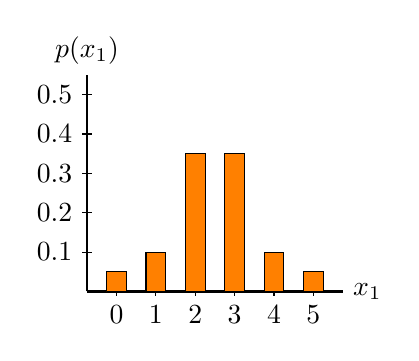
\begin{tikzpicture}
    [scale=0.25]
    %axes
    \draw[thick](0,0)--(0,11) node[above]{$p(x_1)$};
    \draw[thick](0,0)--(13,0) node[right]{$x_1$};
    %label horizontal axis
    \draw (1.5,0.25)--(1.5,-0.25) node[below]{$0$};
    \draw (3.5,0.25)--(3.5,-0.25) node[below]{$1$};
    \draw (5.5,0.25)--(5.5,-0.25) node[below]{$2$};
    \draw (7.5,0.25)--(7.5,-0.25) node[below]{$3$};
    \draw (9.5,0.25)--(9.5,-0.25)
    node[below]{$4$};
    \draw (11.5,0.25)--(11.5,-0.25)
    node[below]{$5$};
    %label vertical axis
    \draw (0.25,2)--(-0.25,2) node[left]{$0.1$};
    \draw (0.25,4)--(-0.25,4) node[left]{$0.2$};
    \draw (0.25,6)--(-0.25,6) node[left]{$0.3$};
    \draw (0.25,8)--(-0.25,8) node[left]{$0.4$};
    \draw (0.25,10)--(-0.25,10) node[left]{$0.5$};
    %histogram
    \draw[fill=orange] (1,0)--(2,0)--(2,1)--(1,1)--(1,0);
    \draw[fill=orange] (3,0)--(3,2)--(4,2)--(4,0)--(3,0);
    \draw[fill=orange] (5,0)--(5,7)--(6,7)--(6,0)--(5,0);
    \draw[fill=orange] (7,0)--(8,0)--(8,7)--(7,7)--(7,0);
    \draw[fill=orange] (9,0)--(10,0)--(10,2)--(9,2)--(9,0);
    \draw[fill=orange]
    (11,0)--(12,0)--(12,1)--(11,1)--(11,0);
    \end{tikzpicture}
&
    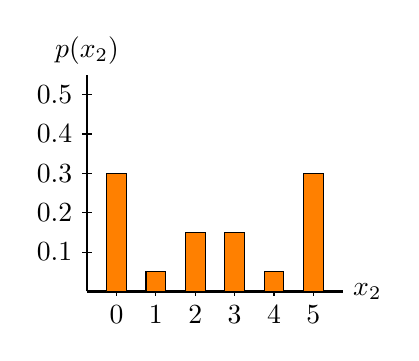
\begin{tikzpicture}
    [scale=0.25]
    %axes
    \draw[thick](0,0)--(0,11) node[above]{$p(x_2)$};
    \draw[thick](0,0)--(13,0) node[right]{$x_2$};
    %label horizontal axis
    \draw (1.5,0.25)--(1.5,-0.25) node[below]{$0$};
    \draw (3.5,0.25)--(3.5,-0.25) node[below]{$1$};
    \draw (5.5,0.25)--(5.5,-0.25) node[below]{$2$};
    \draw (7.5,0.25)--(7.5,-0.25) node[below]{$3$};
    \draw (9.5,0.25)--(9.5,-0.25)
    node[below]{$4$};
    \draw (11.5,0.25)--(11.5,-0.25)
    node[below]{$5$};
    %label vertical axis
    \draw (0.25,2)--(-0.25,2) node[left]{$0.1$};
    \draw (0.25,4)--(-0.25,4) node[left]{$0.2$};
    \draw (0.25,6)--(-0.25,6) node[left]{$0.3$};
    \draw (0.25,8)--(-0.25,8) node[left]{$0.4$};
    \draw (0.25,10)--(-0.25,10) node[left]{$0.5$};
    %histogram
    \draw[fill=orange] (1,0)--(2,0)--(2,6)--(1,6)--(1,0);
    \draw[fill=orange] (3,0)--(3,1)--(4,1)--(4,0)--(3,0);
    \draw[fill=orange] (5,0)--(5,3)--(6,3)--(6,0)--(5,0);
    \draw[fill=orange] (7,0)--(8,0)--(8,3)--(7,3)--(7,0);
    \draw[fill=orange] (9,0)--(10,0)--(10,1)--(9,1)--(9,0);
    \draw[fill=orange]
    (11,0)--(12,0)--(12,6)--(11,6)--(11,0);
    \end{tikzpicture}
&
    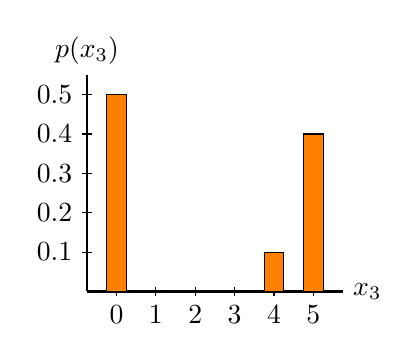
\begin{tikzpicture}
    [scale=0.25]
    %axes
    \draw[thick](0,0)--(0,11) node[above]{$p(x_3)$};
    \draw[thick](0,0)--(13,0) node[right]{$x_3$};
    %label horizontal axis
    \draw (1.5,0.25)--(1.5,-0.25) node[below]{$0$};
    \draw (3.5,0.25)--(3.5,-0.25) node[below]{$1$};
    \draw (5.5,0.25)--(5.5,-0.25) node[below]{$2$};
    \draw (7.5,0.25)--(7.5,-0.25) node[below]{$3$};
    \draw (9.5,0.25)--(9.5,-0.25)
    node[below]{$4$};
    \draw (11.5,0.25)--(11.5,-0.25)
    node[below]{$5$};
    %label vertical axis
    \draw (0.25,2)--(-0.25,2) node[left]{$0.1$};
    \draw (0.25,4)--(-0.25,4) node[left]{$0.2$};
    \draw (0.25,6)--(-0.25,6) node[left]{$0.3$};
    \draw (0.25,8)--(-0.25,8) node[left]{$0.4$};
    \draw (0.25,10)--(-0.25,10) node[left]{$0.5$};
    %histogram
    \draw[fill=orange] (1,0)--(2,0)--(2,10)--(1,10)--(1,0);
    \draw[fill=orange] (3,0)--(3,0)--(4,0)--(4,0)--(3,0);
    \draw[fill=orange] (5,0)--(5,0)--(6,0)--(6,0)--(5,0);
    \draw[fill=orange] (7,0)--(8,0)--(8,0)--(7,0)--(7,0);
    \draw[fill=orange] (9,0)--(10,0)--(10,2)--(9,2)--(9,0);
    \draw[fill=orange]
    (11,0)--(12,0)--(12,8)--(11,8)--(11,0);
    \end{tikzpicture}
\end{tabular}
\end{center}

\begin{itemize}
\item[(a)] Before computing anything and basing your answer solely on the PMF above, put the variances of the three random variables in order from least to greatest. Explain your reasoning.

\vfill

\item[(b)] Sketch an example of a histogram representing the PMF of a random variable $Y$ having {\bf higher} variance than $X_3$. Sketch an example of a histogram representing the PMF of a random variable $Z$ having the same mean as $X_1$ but {\bf lower} variance than $X_1$.\\

\end{itemize}

\,\hfill
%
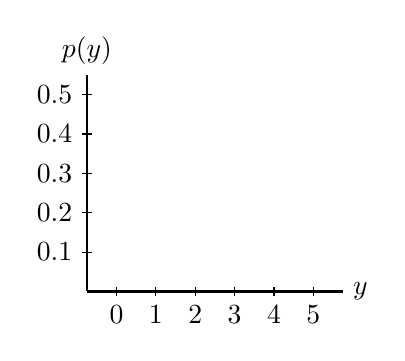
\begin{tikzpicture}
    [scale=0.25]
    %axes
    \draw[thick](0,0)--(0,11) node[above]{$p(y)$};
    \draw[thick](0,0)--(13,0) node[right]{$y$};
    %label horizontal axis
    \draw (1.5,0.25)--(1.5,-0.25) node[below]{$0$};
    \draw (3.5,0.25)--(3.5,-0.25) node[below]{$1$};
    \draw (5.5,0.25)--(5.5,-0.25) node[below]{$2$};
    \draw (7.5,0.25)--(7.5,-0.25) node[below]{$3$};
    \draw (9.5,0.25)--(9.5,-0.25)
    node[below]{$4$};
    \draw (11.5,0.25)--(11.5,-0.25)
    node[below]{$5$};
    %label vertical axis
    \draw (0.25,2)--(-0.25,2) node[left]{$0.1$};
    \draw (0.25,4)--(-0.25,4) node[left]{$0.2$};
    \draw (0.25,6)--(-0.25,6) node[left]{$0.3$};
    \draw (0.25,8)--(-0.25,8) node[left]{$0.4$};
    \draw (0.25,10)--(-0.25,10) node[left]{$0.5$};
    %histogram
    %\draw[fill=orange] (1,0)--(2,0)--(2,10)--(1,10)--(1,0);
    %\draw[fill=orange] (3,0)--(3,0)--(4,0)--(4,0)--(3,0);
    %\draw[fill=orange] (5,0)--(5,0)--(6,0)--(6,0)--(5,0);
    %\draw[fill=orange] (7,0)--(8,0)--(8,0)--(7,0)--(7,0);
    %\draw[fill=orange] (9,0)--(10,0)--(10,2)--(9,2)--(9,0);
    %\draw[fill=orange]
    (11,0)--(12,0)--(12,8)--(11,8)--(11,0);
\end{tikzpicture}
%
\hfill
%
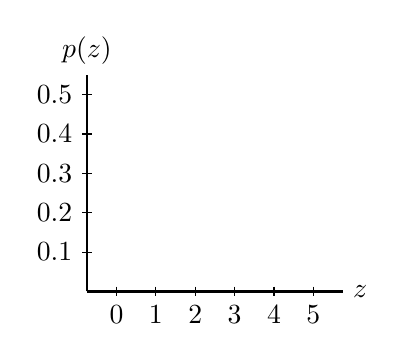
\begin{tikzpicture}
    [scale=0.25]
    %axes
    \draw[thick](0,0)--(0,11) node[above]{$p(z)$};
    \draw[thick](0,0)--(13,0) node[right]{$z$};
    %label horizontal axis
    \draw (1.5,0.25)--(1.5,-0.25) node[below]{$0$};
    \draw (3.5,0.25)--(3.5,-0.25) node[below]{$1$};
    \draw (5.5,0.25)--(5.5,-0.25) node[below]{$2$};
    \draw (7.5,0.25)--(7.5,-0.25) node[below]{$3$};
    \draw (9.5,0.25)--(9.5,-0.25)
    node[below]{$4$};
    \draw (11.5,0.25)--(11.5,-0.25)
    node[below]{$5$};
    %label vertical axis
    \draw (0.25,2)--(-0.25,2) node[left]{$0.1$};
    \draw (0.25,4)--(-0.25,4) node[left]{$0.2$};
    \draw (0.25,6)--(-0.25,6) node[left]{$0.3$};
    \draw (0.25,8)--(-0.25,8) node[left]{$0.4$};
    \draw (0.25,10)--(-0.25,10) node[left]{$0.5$};
    %histogram
    %\draw[fill=orange] (1,0)--(2,0)--(2,10)--(1,10)--(1,0);
    %\draw[fill=orange] (3,0)--(3,0)--(4,0)--(4,0)--(3,0);
    %\draw[fill=orange] (5,0)--(5,0)--(6,0)--(6,0)--(5,0);
    %\draw[fill=orange] (7,0)--(8,0)--(8,0)--(7,0)--(7,0);
    %\draw[fill=orange] (9,0)--(10,0)--(10,2)--(9,2)--(9,0);
    %\draw[fill=orange]
    (11,0)--(12,0)--(12,8)--(11,8)--(11,0);
\end{tikzpicture}
%
\hfill\,

\begin{center}
({\bf Note:} don't forget that the total probability must be exactly 1.)
\end{center}

\hrulefill\\

\begin{center}
({\it Expectation \& Variance of Continuous Random Variables})
\end{center}

\,\hfill \fbox{$\mu=E[X] = \displaystyle\int_{S_X} x\cdot p(x)\,dx$} \hfill\,

\,\hfill \fbox{$Var(X) = E[X^2]-\mu^2=\displaystyle\int_{S_X} x^2\cdot p(x)\,dx-\mu^2$}\hfill\,

Note: You might see elsewhere that the official definition of variance is $Var(X)=\displaystyle\int_{S_X}(x-\mu)^2p(x)\,dx$. The formula boxed above is different from but equivalent to the definition.

%\,\hfill \fbox{$Var(X) = \displaystyle\int_{S_X} (x-\mu)^2\cdot p(x)\,dx$} \fbox{$Var(X) = E[X^2]-\mu^2=\displaystyle\int_{S_X} x^2\cdot p(x)\,dx-\mu^2$}\hfill\,

\exercise\ltrm{\bf\color{Orange}P2} Let the continuous random variable $V$ have the following PDF:
\[
p(v) = 
\begin{cases} 
\frac{1}{v} & \text{for } 1 \leq v \leq e, \\
0 & \text{otherwise}.
\end{cases}
\]

\begin{itemize}
\item[(a)] Find the mean of $V$.
    \vfill

%%%%%%%%%
\newpage%
%%%%%%%%%

\item[(b)] Find the variance of $V$.
    \vfill
    \vfill
    \vfill
\end{itemize}

\exercise\ltrm{\bf\color{Orange}P2} The integral $\dint_1^{c} \frac12z\,dz$ represents the expected value of a random variable $Z$, where $c$ is a constant to be determined.\\

\begin{itemize}
\item[(a)] Find the PDF of $Z$.

\vfill
\item[(b)] Find the value of $c$.

    \vfill
    \vfill

\item[(c)] Find the variance of $Z$.

    \vfill
    \vfill

\end{itemize}

%%%%%%%%%
%\newpage%
%%%%%%%%%

% {\bf\color{blue}Extra Practice 1.} \ltrm{{\bf\color{Orange}P1}}
% Consider a random variable \(X\) that takes integer values from 1 to 5 with frequencies as shown in the histogram below:

% \begin{center}
% \begin{minipage}[t]{0.45\textwidth}
% \,\\[-0.2in]
% \begin{tikzpicture}
%   \begin{axis}[
%       ybar,
%       xlabel={\(X\)},
%       ylabel={Frequency},
%       ymin=0,
%       xmin=0, xmax=6,
%       bar width=0.4,
%       xtick={1,2,3,4,5},
%       nodes near coords,
%       enlargelimits=0.15,
%       title={Histogram Illustrating Frequencies}
%   ]
%   \addplot coordinates {(1,2) (2,3) (3,4) (4,5) (5,1)};
%   \end{axis}
% \end{tikzpicture}
% \end{minipage}
% %
% \quad
% %
% \begin{minipage}[t]{0.45\textwidth}
% \vspace{0.5in}
% \begin{itemize}
%     \item \(X = 1\) has a frequency of 2.
%     \item \(X = 2\) has a frequency of 3.
%     \item \(X = 3\) has a frequency of 4.
%     \item \(X = 4\) has a frequency of 5.
%     \item \(X = 5\) has a frequency of 1.
% \end{itemize}
% \end{minipage}
% \end{center}


% \begin{itemize}
% \item[(a)] Based solely on the histogram above, how are the mean and median of $X$ related? Explain.
%     \vfill

% \item[(b)] Calculate the expected value (mean) of the random variable \(X\). ({\bf Note:} frequencies are given in the histogram above - not probabilities.)
%     \vfill

% \item[(c)] Calculate the median of the random variable $X$. ({\bf Note:} frequencies are given in the histogram above - not probabilities.)
%     \vfill
    
% \end{itemize}

%%%%%%%%%
\newpage%
%%%%%%%%%

{\bf\color{blue}Extra Practice 1.}\ltrm{{\bf\color{Orange}P1}}
Let $X$ be a discrete random variable with the following probability mass function $p(x)$.

\begin{table}[h!]
        \centering
        \begin{tabular}{c|ccccc}
            \hline
           $x$  & 1 & 2 & 3 & 4 & 5\\
           \hline\\
           $p(x)$  & $\dfrac{3}{10}$ & $\dfrac{1}{10}$ & $\dfrac{1}{10}$ & & $\dfrac{3}{10}$\\\\
           \hline
        \end{tabular}
    \end{table}

\begin{enumerate}
    \item[(a)] Find the missing value in the table so that $p(x)$ is a valid probability mass function.

    \item[(b)] Find the expected value of $X$.

    \vfill

    \item[(c)] Find the variance of $x$.
    
    \vfill
\end{enumerate}

%%%%%%%%%
\newpage%
%%%%%%%%%

{\bf\color{blue}Extra Practice 2.}\ltrm{{\bf\color{Orange}P2}}
Compute the expectation of a continuous random variable $W$ with PDF given by:
\[
p(w) = 
\begin{cases} 
2\sqrt{w} & \text{for } 0 \leq w \leq 1, \\
0 & \text{otherwise}.
\end{cases}
\]

\vfill

{\bf\color{blue}Extra Practice 3.}\ltrm{{\bf\color{Orange}P2}} 
Let $X$ be a continuous random variable with the following PDF:
\[
p(x) = \frac{1}{x \ln(10)} \quad \text{for } 1 \leq x \leq 10, \quad \text{and } 0 \text{ otherwise}.
\]
\begin{itemize}
    \item[(a)] Compute the expectation $\mu=E[X]$.
        \vfill
    \item[(b)] Determine the variance $\text{Var}(X)$. You may leave your answer in terms of $\mu$.
        \vfill
        \vfill
\end{itemize}

\end{document}
%%%%%%%%%%%% END DOCUMENT %%%%%%%%%%%%%%%


\exercise\lt{\bf\color{Orange}P3} In the 2018 video game {\it Super Mario Party}, characters move around a board based on rolling either a standard 6-sided die OR a character-specific 6-sided die. For example, Mario can use either the standard 6-sided die or a 6-sided die whose sides are numbered 1, 3, 3, 3, 5, and 6. Below is a table containing the standard 6-sided die, the character-specific die for 6 characters in the game, and the name of a random variable representing the outcome of rolling that character's die:
\begin{center}
\begin{tabular}{| l | l | l | l | l |}
\hline
Die & Variable & Values & Mean $E[\cdot]$ & Variance $Var(\cdot)$\\
\hline
Standard & $S$ & 1, 2, 3, 4, 5, 6 & & \\
\hline
Mario & $M$ & 1, 3, 3, 3, 5, 6 & & \\
\hline
Luigi & $L$ & 1, 1, 1, 5, 6, 7 & & \\
\hline
Peach & $P$ & 0, 2, 4, 4, 4, 6 & & \\
\hline
Daisy & $D$ & 3, 3, 3, 3, 4, 4 & & \\
\hline
Yoshi & $Y$ & 0, 1, 3, 5, 5, 7 & & \\
\hline
Shy Guy & $G$ & 0, 4, 4, 4, 4, 4 & &\\
\hline
\end{tabular}
\end{center}

\begin{itemize}
\item[(a)] ({\bf\color{blue}Group Activity}) Assuming each side of the die is just as likely as the other sides to be turned up, find the mean and variance of $S$, $M$, $L$, $P$, $D$, $Y$, and $G$. Round all answers to two decimal places, as needed.
    \vfill
    \vfill

\item[(b)] ({\bf\color{blue}Discussion}) Usually, players who can reliably move furthest around the board are at an advantage. Of the 7 die above, which one do you think is best, based on their means \& variances (while ignoring other gameplay mechanics)? Explain.
    \vfill
    
\end{itemize}
